\chapter{Adminsitración}
\label{capadministracion}

La capa de Administración de VirtShell proporciona una infraestructura de servicios para la gestión de cualquier dispositivo registrado en el sistema. Este capitulo busca darle explicación a las funcionalidades de administración para utilizarlas en su beneficio.

\section{Particiones, anfitriones y Ambientes en VirtShell}
En VirtShell hay tres conceptos que son muy importantes y se extiende a través de todos los servicios, y que simplemente no puede dejar de tener en cuenta: Las particiones, los ambientes y las instancias. Las tres se asocian con la mayoría de las cosas en VirtShell, y el dominio de ellos es crucial para una buena administración de los dispositivos. 

\subsection{Particiones}
Las particiones consisten de uno o más anfitriones, los cuales pueden ser nodos físicos, servidores o incluso máquinas virtuales. El objetivo principal que busca una partición, es organizar las máquinas que albergaran recursos virtuales en partes aisladas de las demás. Estas partes pueden pueden estar ubicadas en un mismo sitio físico o por el contrario puede estar distribuidas es diferentes zonas geográficas de todo el mundo.\\
\\
Si solo se cuenta con un numero fijo de maquinas (o anfitriones) ubicadas en un mismo sitio físico como por ejemplo un datacenter, lo que se obtiene con las particiones es la posibilidad de dividir esas maquinas en subgrupos que puedan ser destinados para diferentes equipos o divisiones dentro de una organización.\\ 
\\
Al contar con maquinas distribuidas en diferentes zonas geográficas la elección de una partición u otra se basa principalmente en la cercanía de los visitantes o clientes, ya que a menor distancia entre los servidores y ellos, menores son los tiempos de respuesta y mejor la experiencia de usuario.\\
\\
Cuando se crea una nueva partición, VirtShell la crea completamente vaciá, sin anfitriones. Para asociar anfitriones a una partición se debe crear un anfitrión y vincularlo con la partición como se vera mas adelante en este mismo capitulo. Un ejemplo de como crear una partición usando el API se muestra en el siguiente código:

\begin{lstlisting}[style=json, caption=Petición HTTP para crear una partición]
curl -sv -X POST \
  -H 'accept: application/json' \
  -H 'X-VirtShell-Authorization: UserId:Signature' \
  -d '{
  	   "name": "development_co",
       "description": "Collection of servers oriented to development team in colombia."
      }' \
   'http://localhost:8080/api/virtshell/v1/partitions'
\end{lstlisting}


\subsection{Asociación de anfitriones a particiones}
Los anfitriones no son mas que nodos físicos, servidores o máquinas virtuales, que alojaran recursos virtuales. VirtShell ofrece la posibilidad de clasificarlos de acuerdo a combinaciones de capacidad de CPU, memoria, almacenamiento y red. El objetivo que busca la clasificación es proporcionar flexibilidad para elegir la combinación de recursos adecuada para las aplicaciones.\\
\\
Los tipos de anfitriones se agrupan en familias basadas en perfiles de aplicación de destino. Estos grupos incluyen: de propósito general, con procesadores de alto desempeño, de memoria optimizada, de almacenamiento optimizado.

\begin{description}
\item [Propósito general] Esta familia proporciona un equilibrio de recursos informáticos, de memoria y red, por lo que constituye una buena opción para muchas aplicaciones.
\item [Procesadores de alto desempeño] Esta familia ofrece procesadores que alcanzan alto desempeño en tareas complejas.
\item [Memoria optimizada] Esta familia esta optimizada para aplicaciones con un uso intenso de la memoria.
\item [Almacenamiento optimizado] Esta familia promete anfitriones con alta capacidad de almacenamiento, optimizado para un desempeño de E/S muy alto.
\end{description}

Cuando se crea un anfitrión en VirtShell este debe ser asociado a una sola partición, asignándole un tipo, con alguno de los mencionados anteriormente, estableciendo las capacidad de disco y memoria RAM con las que cuenta,  
indicando también el sistema operativo y las ip con las que se conecta a la red. Una vez el anfitrión es creado en el sistema este queda asignado a la partición elegida. El siguiente ejemplo muestra como crear un anfitrión usando el API:

\begin{lstlisting}[style=json, caption=Petición HTTP para crear un host]
curl -sv -X POST \
  -H 'accept: application/json' \
    -H 'X-VirtShell-Authorization: UserId:Signature' \
  -d '{"name": "host-01-pdn",
       "os": "Ubuntu_12.04_3.5.0-23.x86_64",
       "memory": "16GB",
       "capacity": "120GB",
       "enabled": "true",
       "type" : "GeneralPurpose",
       "local_ipv4": "15.54.88.19",
       "local_ipv6": "ff06:0:0:0:0:0:0:c3",
       "public_ipv4": "10.54.88.19",
       "public_ipv6": "yt06:0:0:0:0:0:0:c3",
       "partition": "development_co"}' \
   'http://localhost:8080/virtshell/api/v1/hosts'
\end{lstlisting}

En este ejemplo se muestra la creación de un host con nombre host-01-pdn que esta clasificado como de uso general y que queda asociado a la partición development\_co creada en la sección anterior.\\
\\
Al consultar la partición nuevamente por medio del API se puede observar como el anfitrión se encuentra asociado a la partición developtment\_co. En la siguiente consulta al API se muestra el resultado de la asociación: 

\begin{lstlisting}[style=json, , caption=Petición HTTP para consultar una partición por su nombre]
curl -sv -H 'accept: application/json' 
     -H 'X-VirtShell-Authorization: UserId:Signature' \ 
     'http://<host>:<port>/api/virtshell/v1/partitions/development_co'
\end{lstlisting}

Response:

\begin{lstlisting}[style=json]
HTTP/1.1 200 OK
Content-Type: application/json
{
  "uuid": "efa1777c-cad7-11e5-9956-625662870761",
  "name": "development_co",
  "description": "Collection of servers oriented to development team in colombia.", 
  "hosts": [ "host-01-pdn" ],  
  "created": {"at":"1429207233", 
              "by":"1a900cdc-cad8-11e5-9956-625662870761"}
}
\end{lstlisting}

Adicionalmente, cuando un anfitrión es agregado a una partición, VirtShell instala automáticamente los agentes  que realizaran tareas de aprovisionamiento y monitoreo. Los agentes se explicaran mas adelante.

\subsection{División de particiones en ambientes}
Las particiones se refieren a la forma de organizar lugares físicos. Los ambientes por el contrario, son lugares lógicos y aislados dentro de una partición. Cada partición puede estar compuesta por uno o varios ambientes. Cada ambiente pertenece a una sola partición. La figura \ref{fig:enviroment} muestra un ejemplo de como dos particiones contiene varios ambientes destinados a equipos de trabajo diferentes. \\

\begin{figure}[h]
    \centering
	\caption{Ejemplo de ambientes en un partición}
	\label{fig:enviroment}
	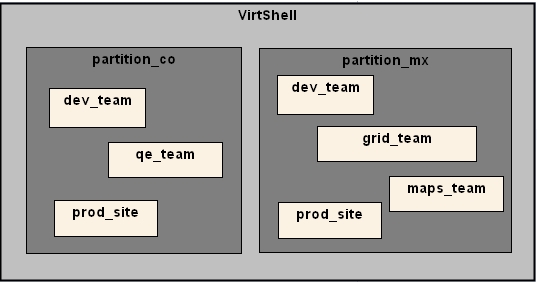
\includegraphics[width = 0.95\textwidth]{../architecture/v1/diagrams/enviroments}
\end{figure}

Un ejemplo de como crear un ambiente asociado a una partición usando el API se muestra en el siguiente código:

\begin{lstlisting}[style=json, caption=Petición HTTP para crear un ambiente]
curl -sv -X POST \
  -H 'accept: application/json' \
  -H 'X-VirtShell-Authorization: UserId:Signature' \
  -d '{
       "name": "bigdata_laboratory",
       "description": "Collection of servers oriented to big data.", 
       "partition": "bogota_partition_co"
      }' \
   'http://localhost:8080/api/virtshell/v1/enviroments'
\end{lstlisting}

\section{Instancias}
A un servidor virtual en VirtShell, se le denomina instancia. Una instancia no es mas que un recurso virtual que se ejecuta sobre un anfitrión. Las instancias pueden ser maquinas virtuales que corren sobre algún hipervisor o también pueden ser contenedores que se ejecutan directamente sobre el sistema operativo del anfitrión.
\\
Las instancias se crean sobre los ambientes de trabajo.
\\
Una buena razón para tener ambientes es la disponibilidad. Si distribuye sus instancias a través de múltiples ambientes y una instancia falla, puede diseñar su aplicación para que una instancia en otra ambiente pueda atender las peticiones. Una especie de equilibrador de carga de emergencia sin necesidad de utilizar un equilibrador de carga real.


